\documentclass{article}
\usepackage{graphicx}
\usepackage[utf8]{inputenc}
\usepackage[T1]{fontenc}
\usepackage{lmodern}
\usepackage{float}
\usepackage{caption}
\usepackage{subcaption}
\usepackage[paperwidth=4.1in, paperheight=5.8in, margin=0.25in]{geometry}
\renewcommand*\familydefault{\sfdefault}
\pagenumbering{gobble}

\usepackage{pgfmorepages}

\pgfpagesdeclarelayout{8 on 2, book format}
{%
  \edef\pgfpageoptionheight{\the\paperheight}
  \edef\pgfpageoptionwidth{\the\paperwidth}
  \def\pgfpageoptionborder{0pt}
  \def\pgfpageoptionfirstshipout{1}
}%
{%
  \pgfpagesphysicalpageoptions
  {%
    logical pages=8,%
    physical pages=2,%
    physical height=\pgfpageoptionheight,%
    physical width=\pgfpageoptionwidth,%
    current logical shipout=\pgfpageoptionfirstshipout%
  }
  \pgfpagesphysicalpage{1}{}
    \pgfpageslogicalpageoptions{4}
    {%
      border shrink=\pgfpageoptionborder,%
      resized width=.5\pgfphysicalwidth,%
      resized height=.5\pgfphysicalheight,%
      center=\pgfpoint{.25\pgfphysicalwidth}{.75\pgfphysicalheight}%
    }%
    \pgfpageslogicalpageoptions{2}
    {%
      border shrink=\pgfpageoptionborder,%
      resized width=.5\pgfphysicalwidth,%
      resized height=.5\pgfphysicalheight,%
      center=\pgfpoint{.75\pgfphysicalwidth}{.75\pgfphysicalheight}%
    }%
    \pgfpageslogicalpageoptions{8}
    {%
      border shrink=\pgfpageoptionborder,%
      resized width=.5\pgfphysicalwidth,%
      resized height=.5\pgfphysicalheight,%
      center=\pgfpoint{.25\pgfphysicalwidth}{.25\pgfphysicalheight},%
    }%
    \pgfpageslogicalpageoptions{6}
    {%
      border shrink=\pgfpageoptionborder,%
      resized width=.5\pgfphysicalwidth,%
      resized height=.5\pgfphysicalheight,%
      center=\pgfpoint{.75\pgfphysicalwidth}{.25\pgfphysicalheight},%
    }%
  \pgfpagesphysicalpage{2}{}
    \pgfpageslogicalpageoptions{1}
    {%
      border shrink=\pgfpageoptionborder,%
      resized width=.5\pgfphysicalwidth,%
      resized height=.5\pgfphysicalheight,%
      center=\pgfpoint{.25\pgfphysicalwidth}{.75\pgfphysicalheight}%
    }%
    \pgfpageslogicalpageoptions{3}
    {%
      border shrink=\pgfpageoptionborder,%
      resized width=.5\pgfphysicalwidth,%
      resized height=.5\pgfphysicalheight,%
      center=\pgfpoint{.75\pgfphysicalwidth}{.75\pgfphysicalheight}%
    }%
    \pgfpageslogicalpageoptions{5}
    {%
      border shrink=\pgfpageoptionborder,%
      resized width=.5\pgfphysicalwidth,%
      resized height=.5\pgfphysicalheight,%
      center=\pgfpoint{.25\pgfphysicalwidth}{.25\pgfphysicalheight},%
    }%
    \pgfpageslogicalpageoptions{7}
    {%
      border shrink=\pgfpageoptionborder,%
      resized width=.5\pgfphysicalwidth,%
      resized height=.5\pgfphysicalheight,%
      center=\pgfpoint{.75\pgfphysicalwidth}{.25\pgfphysicalheight},%
    }%
}


\pgfpagesuselayout{8 on 2, book format}[a4paper]
\begin{document}
    
        \par\noindent\rule{\textwidth}{0.4pt}
    \begin{figure}[H]
        \centering
        \begin{minipage}{0.25\textwidth}
            \centering
            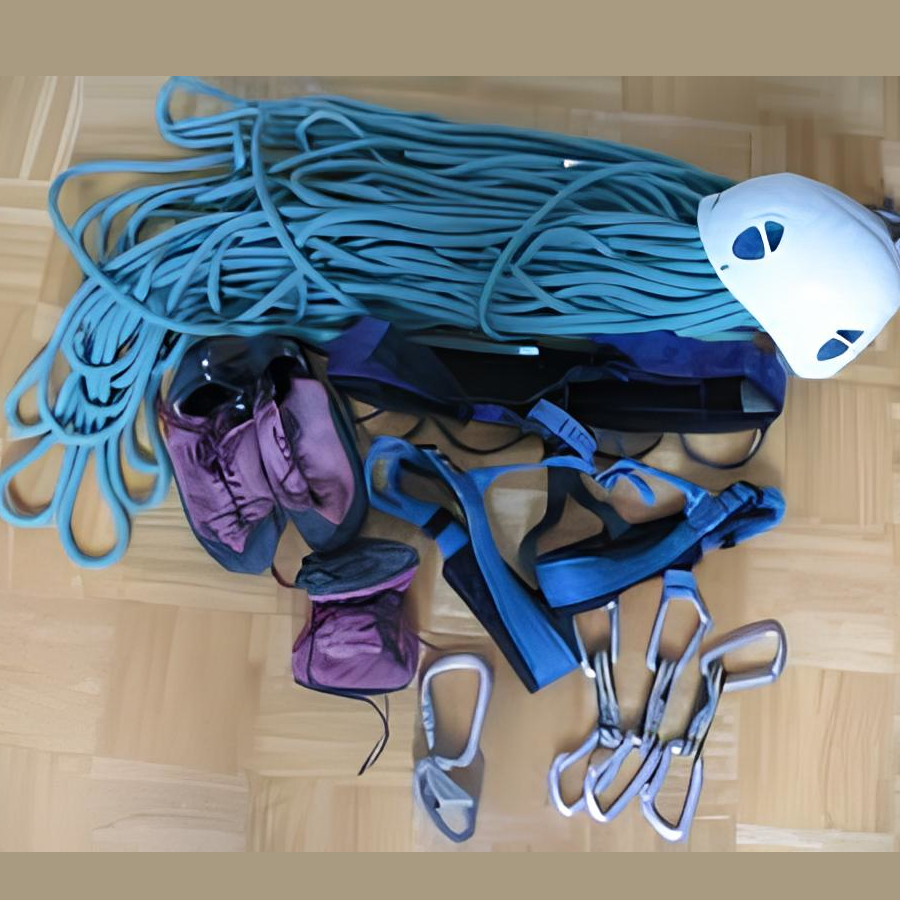
\includegraphics[width=\textwidth]{../SurvivalItemImages/climbinggear}
        \end{minipage}\hfill
        \begin{minipage}{0.7\textwidth}
            \centering
            \Large Climbing gear with reserve helmet
        \end{minipage}
    \end{figure}
    \vspace{-0.8em}
    \noindent\rule{\textwidth}{0.4pt}
            
    \begin{figure}[H]
        \centering
        \begin{minipage}{0.25\textwidth}
            \centering
            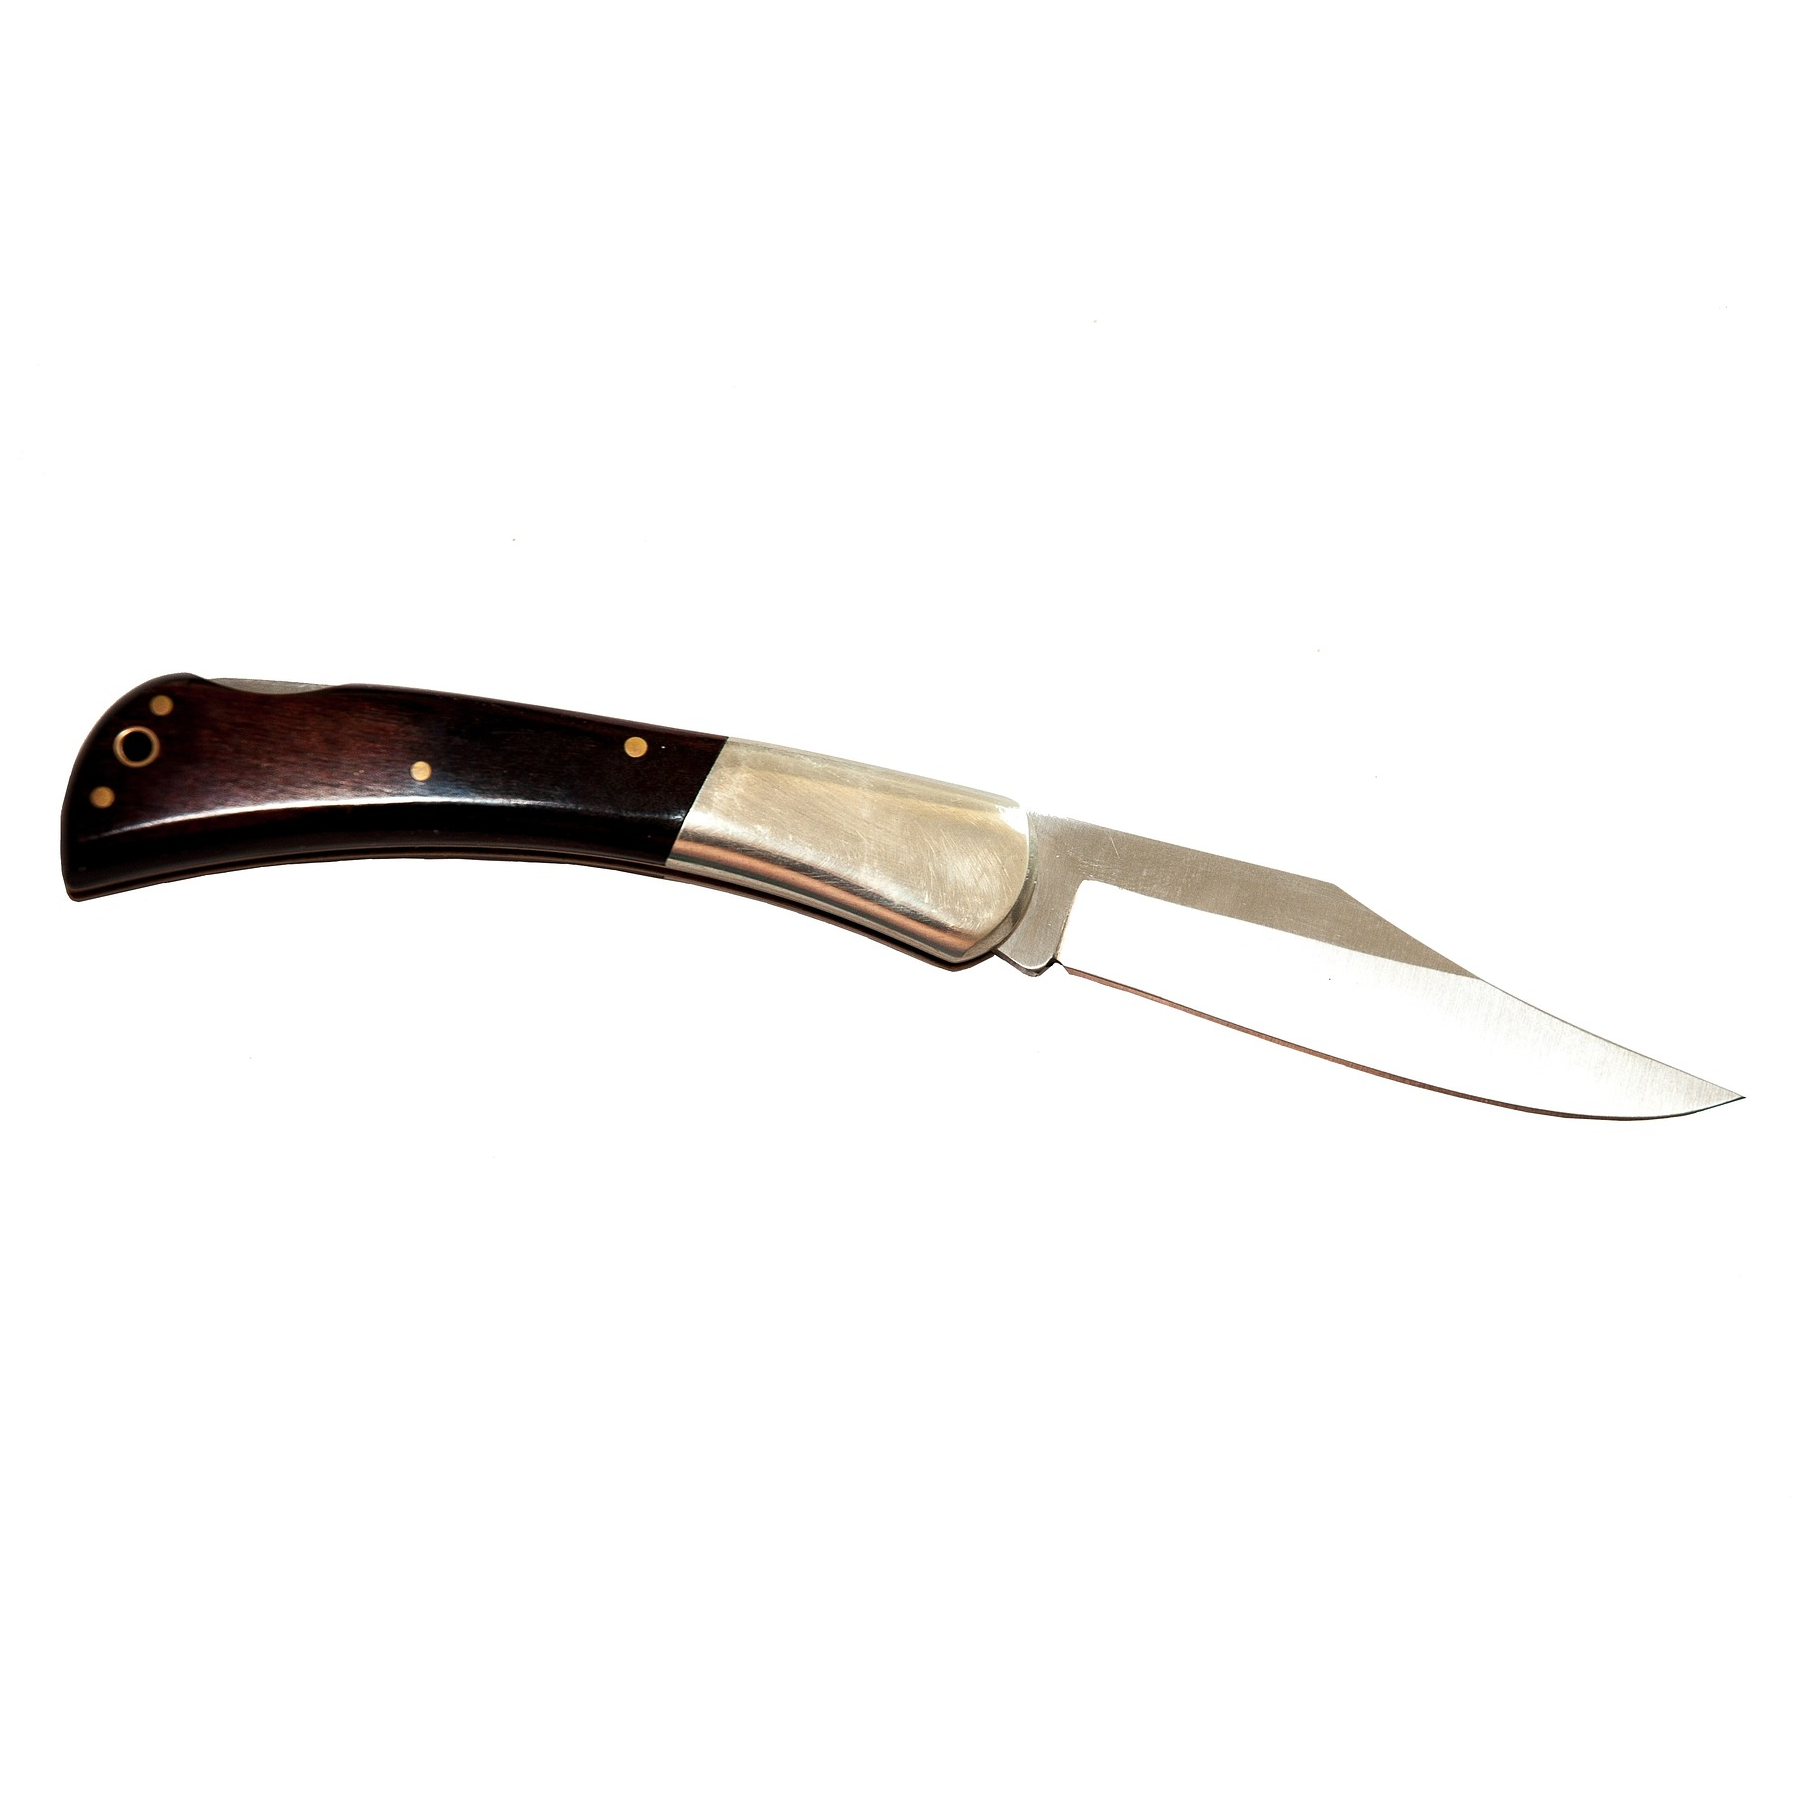
\includegraphics[width=\textwidth]{../SurvivalItemImages/knife}
        \end{minipage}\hfill
        \begin{minipage}{0.7\textwidth}
            \centering
            \Large Folding knife
        \end{minipage}
    \end{figure}
    \vspace{-0.8em}
    \noindent\rule{\textwidth}{0.4pt}
            
    \begin{figure}[H]
        \centering
        \begin{minipage}{0.25\textwidth}
            \centering
            \includegraphics[width=\textwidth]{../SurvivalItemImages/tent}
        \end{minipage}\hfill
        \begin{minipage}{0.7\textwidth}
            \centering
            \Large Camping tent
        \end{minipage}
    \end{figure}
    \vspace{-0.8em}
    \noindent\rule{\textwidth}{0.4pt}
            
    \begin{figure}[H]
        \centering
        \begin{minipage}{0.25\textwidth}
            \centering
            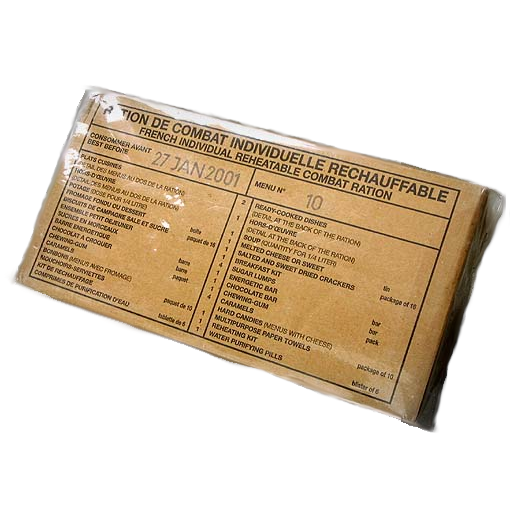
\includegraphics[width=\textwidth]{../SurvivalItemImages/rations}
        \end{minipage}\hfill
        \begin{minipage}{0.7\textwidth}
            \centering
            \Large A case of army rations
        \end{minipage}
    \end{figure}
    \vspace{-0.8em}
    \noindent\rule{\textwidth}{0.4pt}
            
    \clearpage
    \section*{Scenario: \textmd{Mountains} \hfill Participant \textmd{0}}
    \Large On a mountain hike, an avalanche occurred that destroyed most of your base camp. You and two fellow travellers could climb out of the snow. Unfortunately the avalanche carried away your mountain guide and you could not find him. Your base camp is located a three day walk from the next village, on a height which does not require oxygen supply. The weather is good, but you need to expect temperatures below -15° C. You are all wearing winter clothes and mountain boots. Not all of the camping gear was buried: you could find some items.\clearpage
        \par\noindent\rule{\textwidth}{0.4pt}
    \begin{figure}[H]
        \centering
        \begin{minipage}{0.25\textwidth}
            \centering
            \includegraphics[width=\textwidth]{../SurvivalItemImages/kettle}
        \end{minipage}\hfill
        \begin{minipage}{0.7\textwidth}
            \centering
            \Large A camping kettle with mounting
        \end{minipage}
    \end{figure}
    \vspace{-0.8em}
    \noindent\rule{\textwidth}{0.4pt}
            
    \begin{figure}[H]
        \centering
        \begin{minipage}{0.25\textwidth}
            \centering
            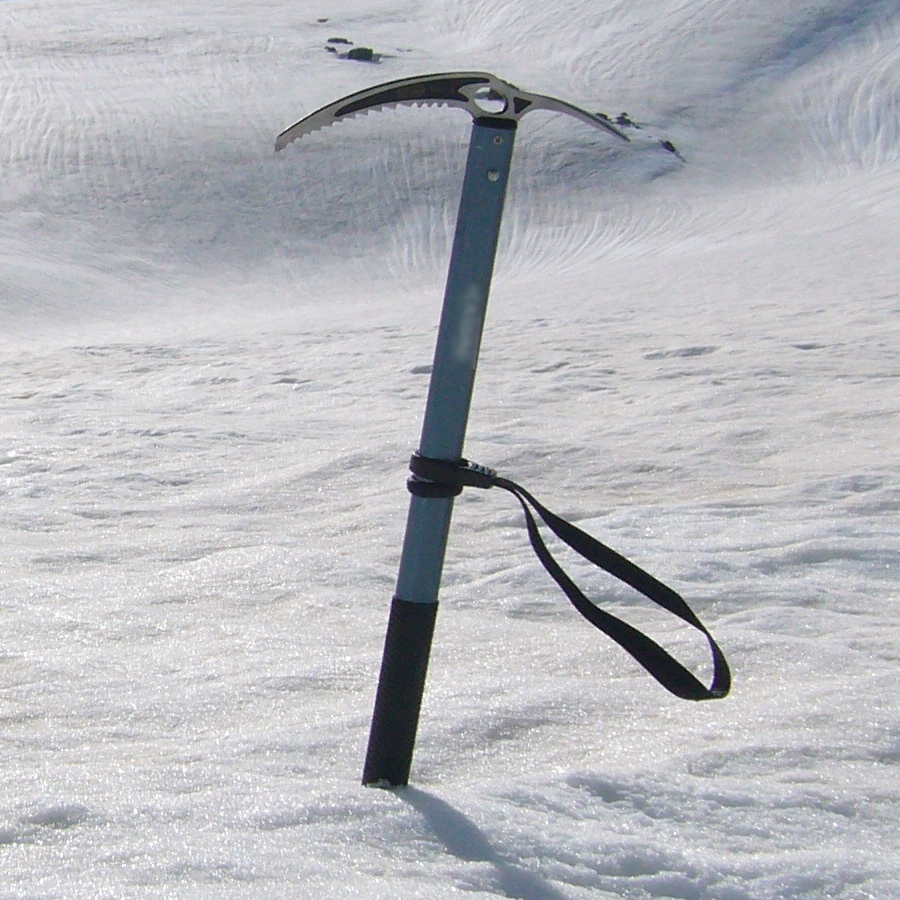
\includegraphics[width=\textwidth]{../SurvivalItemImages/mountainaxe}
        \end{minipage}\hfill
        \begin{minipage}{0.7\textwidth}
            \centering
            \Large A mountaineer's axe
        \end{minipage}
    \end{figure}
    \vspace{-0.8em}
    \noindent\rule{\textwidth}{0.4pt}
            
    \begin{figure}[H]
        \centering
        \begin{minipage}{0.25\textwidth}
            \centering
            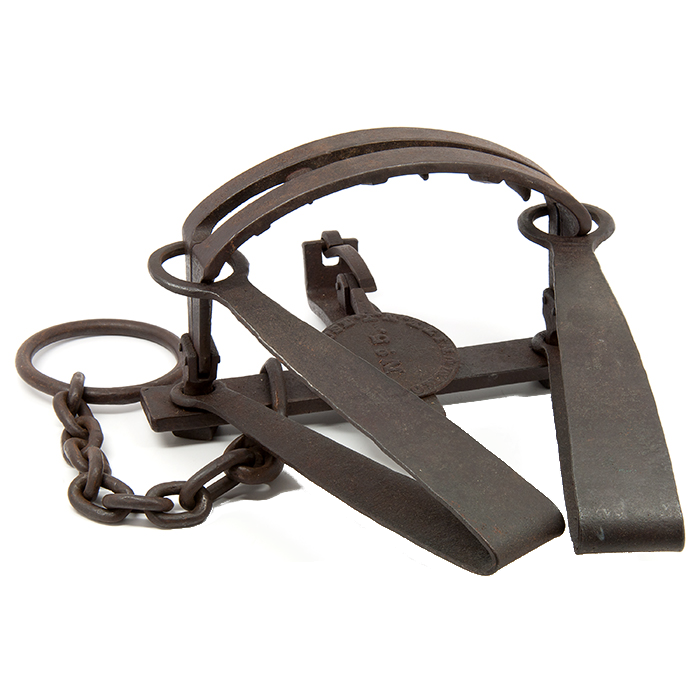
\includegraphics[width=\textwidth]{../SurvivalItemImages/trap}
        \end{minipage}\hfill
        \begin{minipage}{0.7\textwidth}
            \centering
            \Large An animal trapping
        \end{minipage}
    \end{figure}
    \vspace{-0.8em}
    \noindent\rule{\textwidth}{0.4pt}
            
    \begin{figure}[H]
        \centering
        \begin{minipage}{0.25\textwidth}
            \centering
            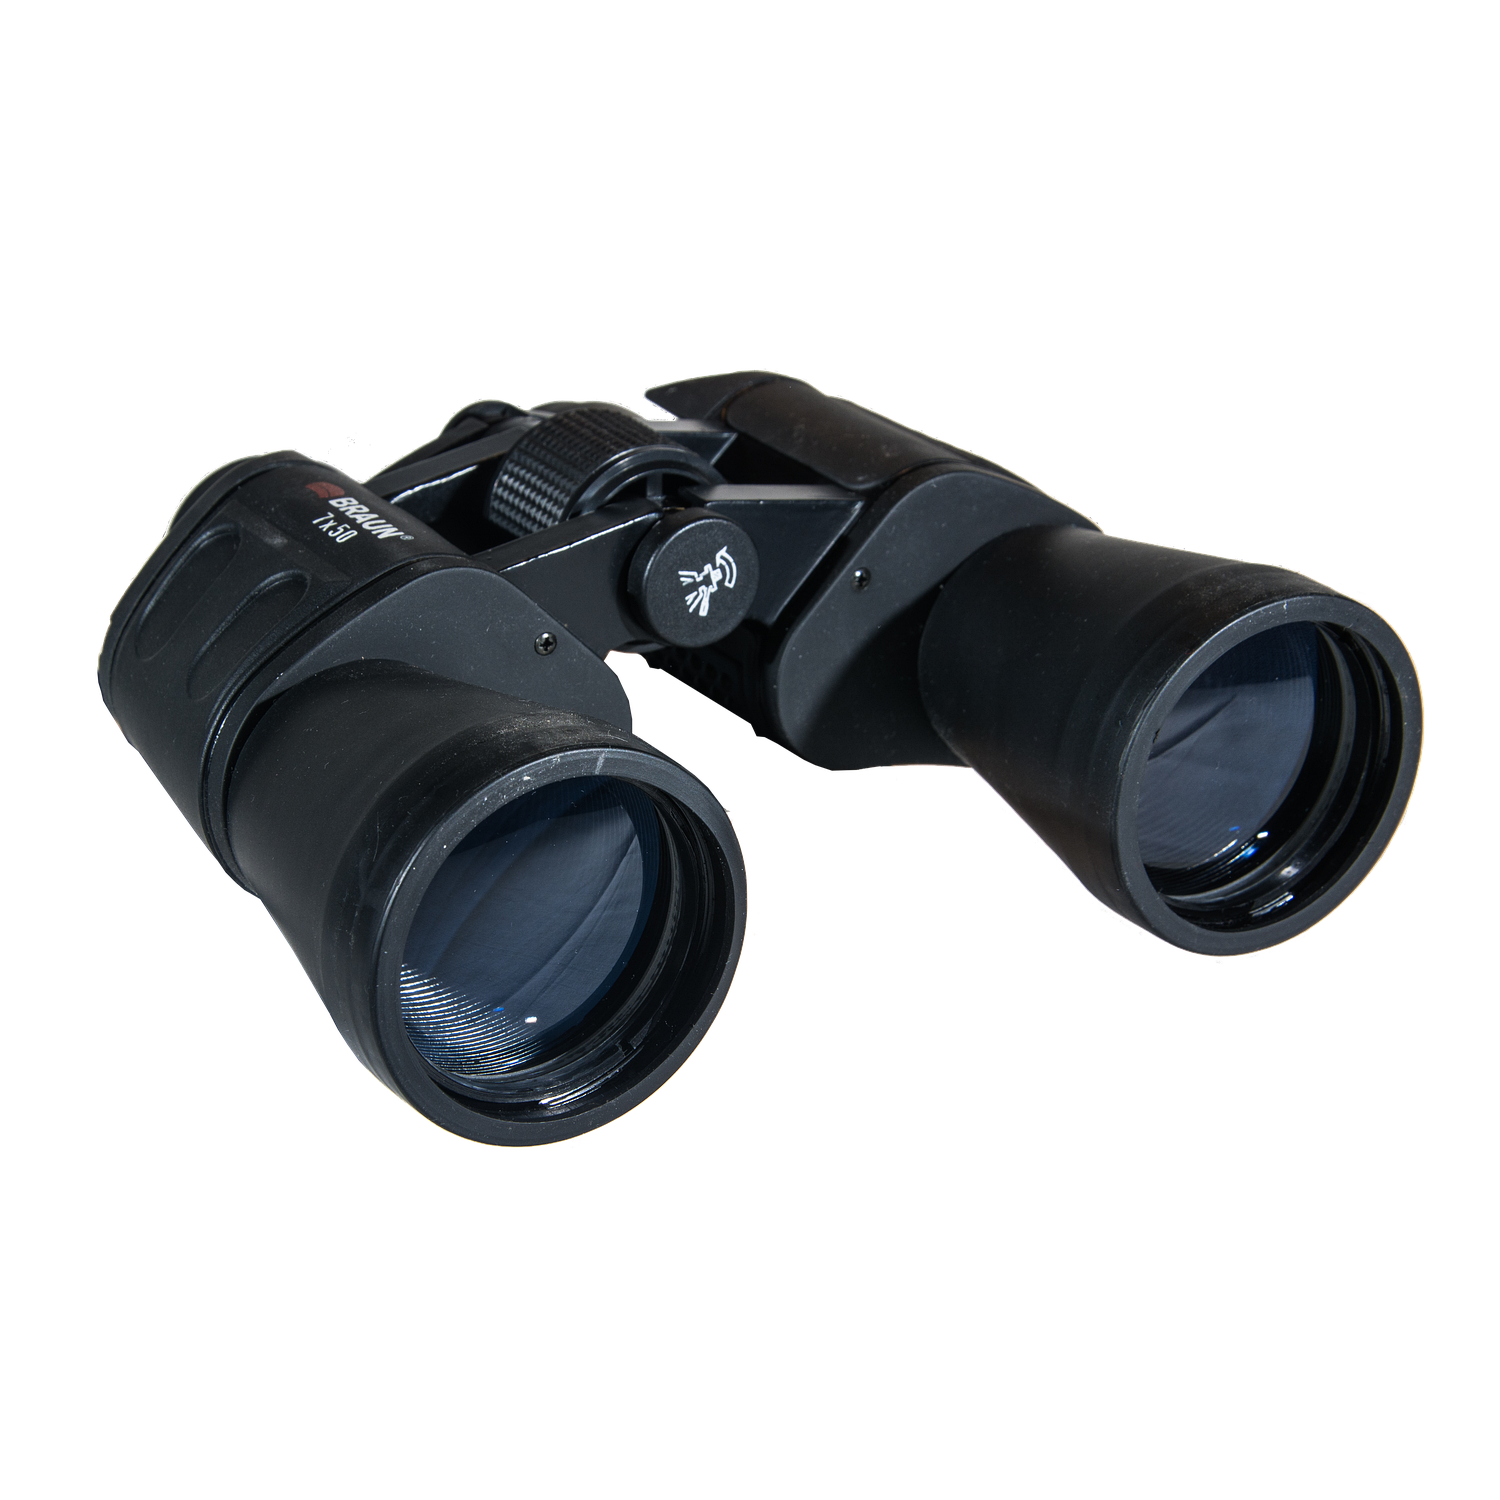
\includegraphics[width=\textwidth]{../SurvivalItemImages/binoculars}
        \end{minipage}\hfill
        \begin{minipage}{0.7\textwidth}
            \centering
            \Large Binoculars
        \end{minipage}
    \end{figure}
    \vspace{-0.8em}
    \noindent\rule{\textwidth}{0.4pt}
            
    \clearpage
    \section*{Scenario: \textmd{Mountains} \hfill Participant \textmd{1}}
    \Large On a mountain hike, an avalanche occurred that destroyed most of your base camp. You and two fellow travellers could climb out of the snow. Unfortunately the avalanche carried away your mountain guide and you could not find him. Your base camp is located a three day walk from the next village, on a height which does not require oxygen supply. The weather is good, but you need to expect temperatures below -15° C. You are all wearing winter clothes and mountain boots. Not all of the camping gear was buried: you could find some items.\clearpage
        \par\noindent\rule{\textwidth}{0.4pt}
    \begin{figure}[H]
        \centering
        \begin{minipage}{0.25\textwidth}
            \centering
            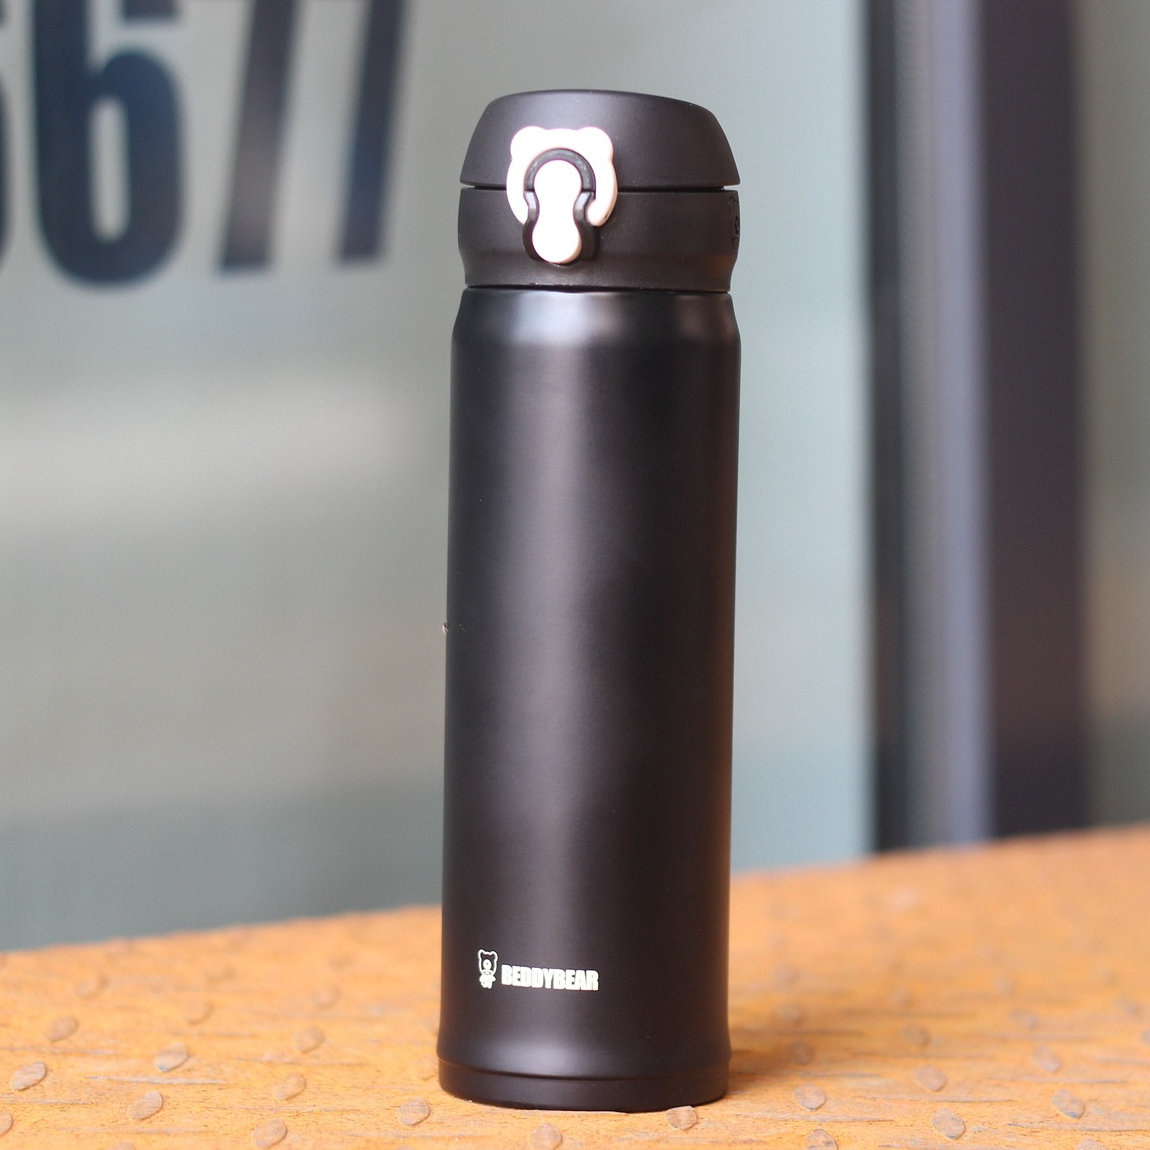
\includegraphics[width=\textwidth]{../SurvivalItemImages/thermos}
        \end{minipage}\hfill
        \begin{minipage}{0.7\textwidth}
            \centering
            \Large A thermos bottle
        \end{minipage}
    \end{figure}
    \vspace{-0.8em}
    \noindent\rule{\textwidth}{0.4pt}
            
    \begin{figure}[H]
        \centering
        \begin{minipage}{0.25\textwidth}
            \centering
            \includegraphics[width=\textwidth]{../SurvivalItemImages/mat}
        \end{minipage}\hfill
        \begin{minipage}{0.7\textwidth}
            \centering
            \Large A sleeping mat
        \end{minipage}
    \end{figure}
    \vspace{-0.8em}
    \noindent\rule{\textwidth}{0.4pt}
            
    \begin{figure}[H]
        \centering
        \begin{minipage}{0.25\textwidth}
            \centering
            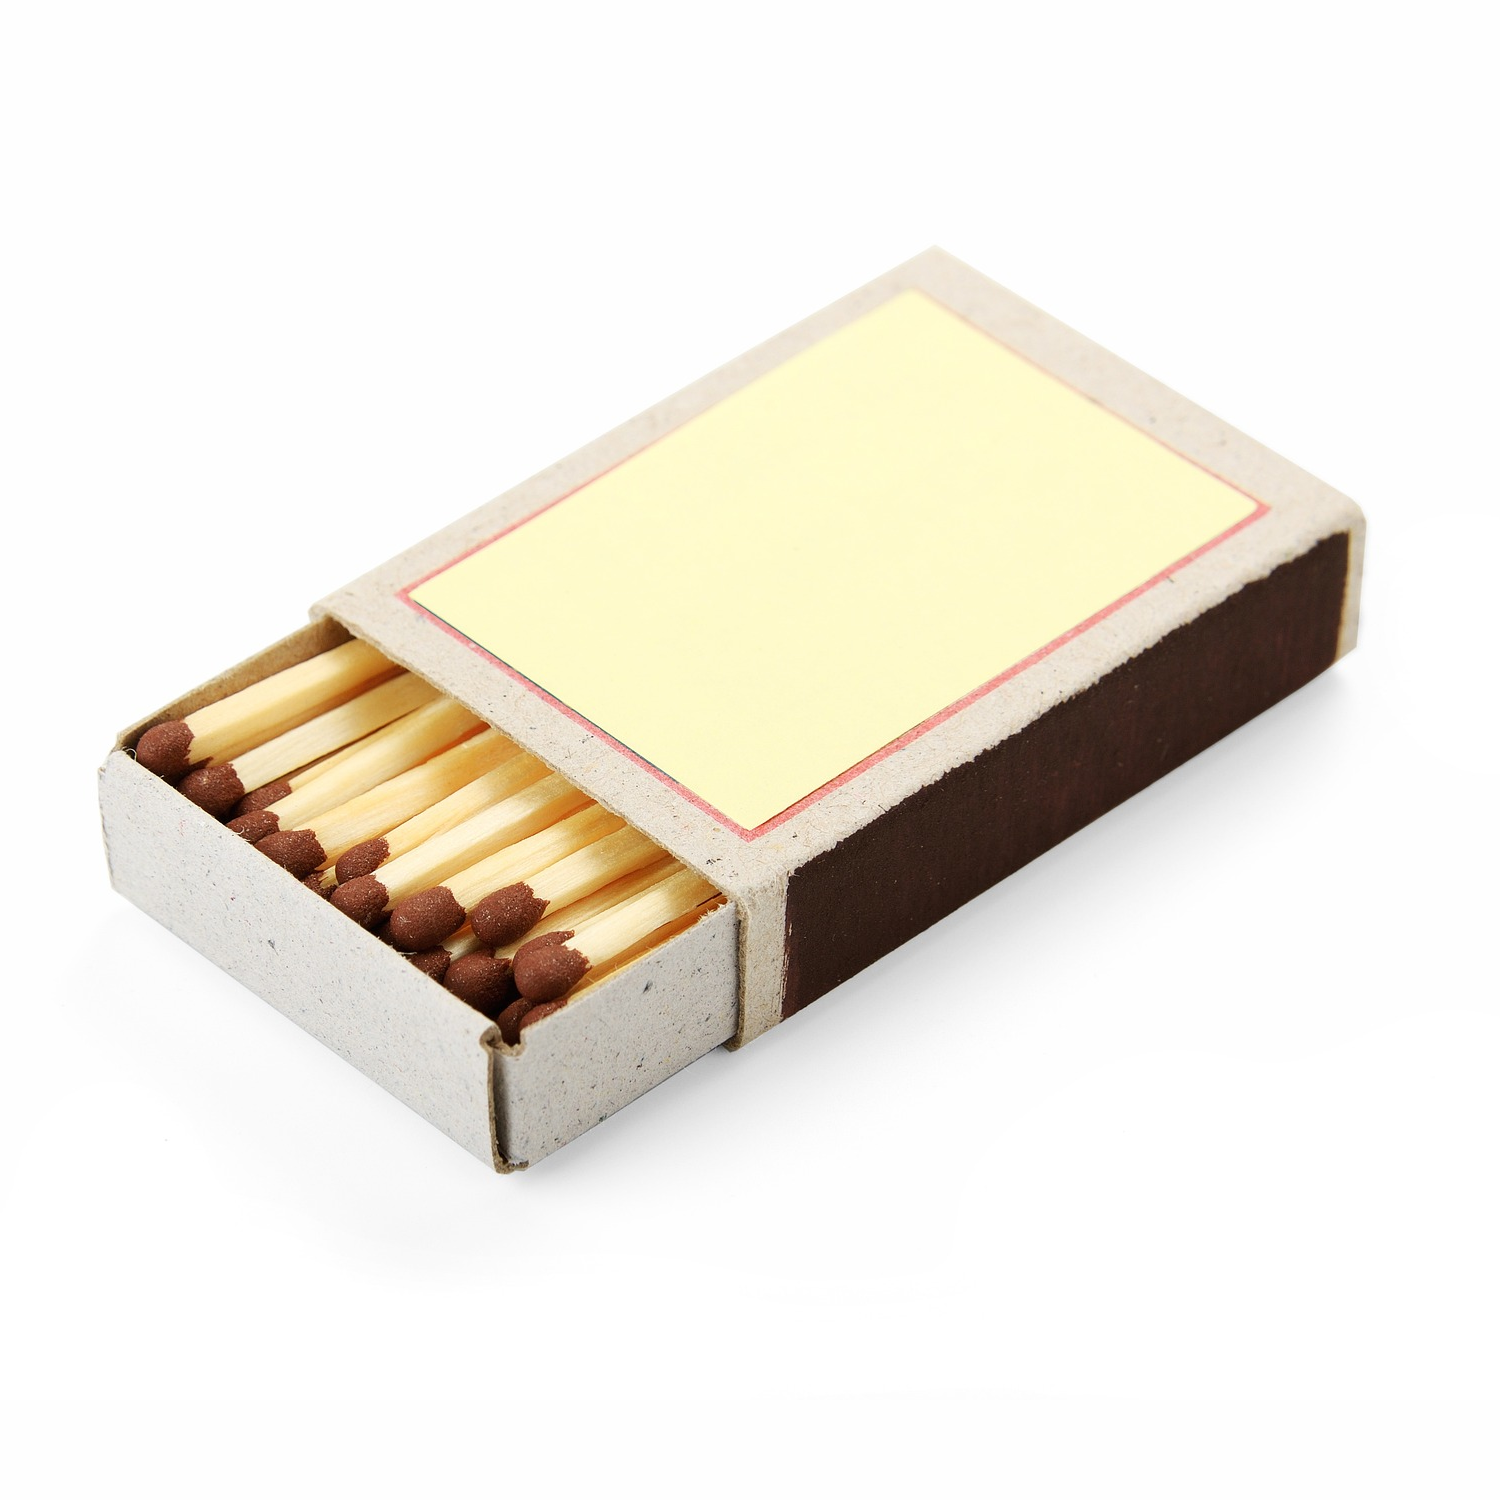
\includegraphics[width=\textwidth]{../SurvivalItemImages/matchbox}
        \end{minipage}\hfill
        \begin{minipage}{0.7\textwidth}
            \centering
            \Large Box of matches
        \end{minipage}
    \end{figure}
    \vspace{-0.8em}
    \noindent\rule{\textwidth}{0.4pt}
            
    \begin{figure}[H]
        \centering
        \begin{minipage}{0.25\textwidth}
            \centering
            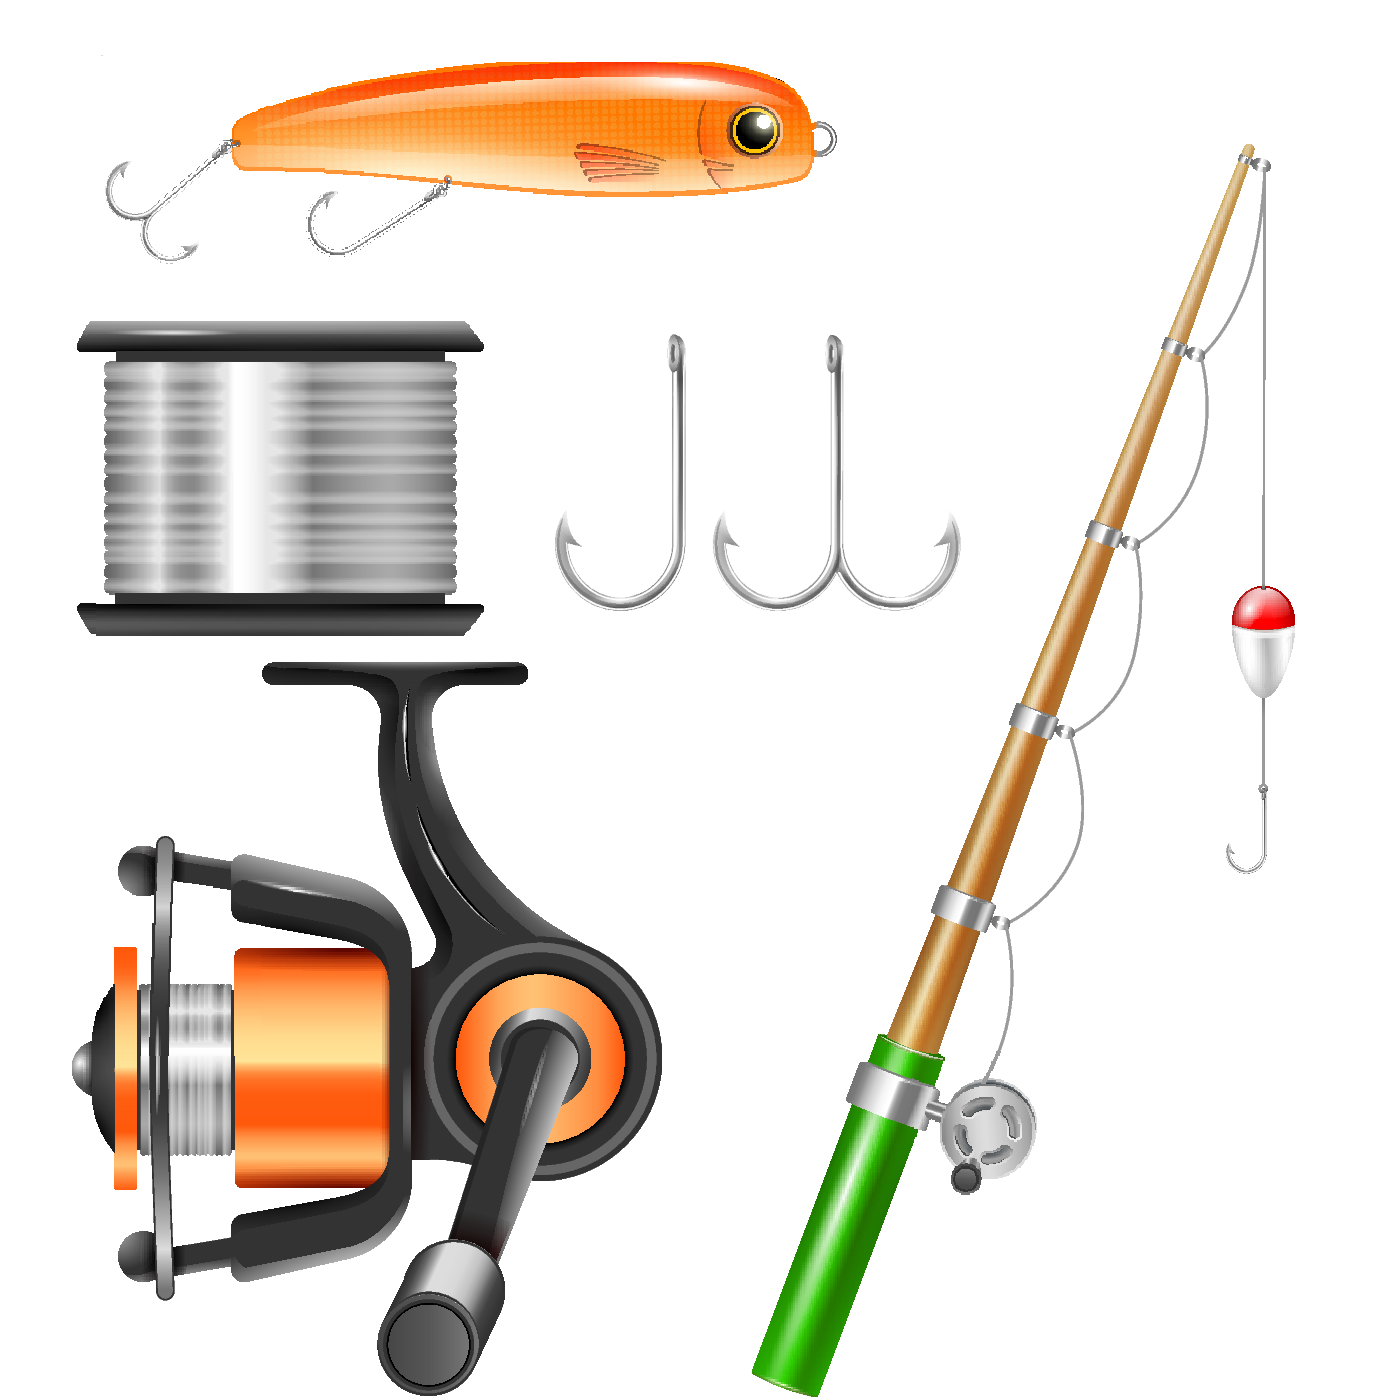
\includegraphics[width=\textwidth]{../SurvivalItemImages/fishingkit}
        \end{minipage}\hfill
        \begin{minipage}{0.7\textwidth}
            \centering
            \Large A fishing kit
        \end{minipage}
    \end{figure}
    \vspace{-0.8em}
    \noindent\rule{\textwidth}{0.4pt}
            
    \clearpage
    \section*{Scenario: \textmd{Mountains} \hfill Participant \textmd{2}}
    \Large On a mountain hike, an avalanche occurred that destroyed most of your base camp. You and two fellow travellers could climb out of the snow. Unfortunately the avalanche carried away your mountain guide and you could not find him. Your base camp is located a three day walk from the next village, on a height which does not require oxygen supply. The weather is good, but you need to expect temperatures below -15° C. You are all wearing winter clothes and mountain boots. Not all of the camping gear was buried: you could find some items.\clearpage
        \end{document}
        